\todo{comments liesel paradigms})
\todo{spellcheck}
\todo{are all acronyms defined}
\todo{fix all latex warnings to make sure no refs are missing (or grep on that
specific warning)}
\todo{uniform ref or autoref}
\todo{don't capitalize figure, table, algorithm,...}
\todo{define short captions for tables and figures}
\todo{fix lacheck/chktex notifications}

People suffering from severe paralysis or disability due to
neurodegenenerative disease, stroke, traumatic brain or spine injury
become entirely reliant on caregivers or family members in their day to day
routine.
Wouldn't it be great if we could help them regain some quality of life by
making them more independent?

The most basic ability any independent human being needs, is interaction with
their environment.
In its core essence, this is the ability to communicate your intentions,
emotions, frustrations or thoughts such that they might be acted on.
For an able-bodied person, physical interaction happens through body movements
while communication is usually done through speech and body language
Both require sending signals through the body's nervous system to control
muscles.
Not everyone has this capability.

The key problem for severely paralyzed patients is that the mind wants to go
where the body can't follow.
Couldn't we therefore design a system that directly interacts with the mind?
This system can then form an interface between the mind and any kind of
technology, like a robot arm or speech synthesizer, interacting with the world
on the user's behalf.
Such a device is the \ac{bci}\footnote{Sometimes also
termed brain-machine interface (BMI) when coupled to a physical actuator, like
a robot arm or an exoskeleton.
The term \ac{bci} is usually preferred for
assistive technology and communication devices.
},
a system that directly couples actions in the `real world' to the mental state of
the user.

Starting in the 1970's from methods to establish basic communication from
minimal brain activity (yes/no, left/right, \ldots)~\cite{Wolpaw2002}, \acp{bci} have gradually evolved
into sophisticated interaction schemes that restore or enhance many capabilities
by bypassing defective parts of the nervous or muscle system.
By now, classic \acp{bci} methods are starting to mature outside the lab
setting and can be used as assistive communication technology by patients with
impaired speech~\cite{Wolpaw2018,Milekovic2018}.
Impressive cutting edge examples of experimental use include a brain-spine
interface allowing a paraplegic patient to walk again\cite{Lorach2023},
a \ac{bci} translating internal speech to a facial avatar speaking the imagined
text~\cite{Metzger2023}, and fast communication through decoding imagined
handwritten symbols~\cite{Willett2021}.
Recently, the idea has also gained popular traction through Elon Musk's
NeuraLink~\cite{Musk2019} initiative, which imagines a multipurpose \ac{bci}.

In general, devices processing direct inputs from the central nervous system
are useful for rehabilitation and medical diagnosis or treatment.
Additionally, they bring a new paradigm to human-computer interaction,
especially when paired with virtual or augmented reality.\todo{cite}
Ultimatly, they have always been especially promising as assistive technology for
paralyzed patients limited in their communication ability.
It is this \ac{bci} controlled communication is where our focus lies,
as it offers a transformative means for individuals with severe motor
impairments to regain functional independence to write and speak through
assistive technology.
This allows them to talk to their loved ones and caregivers, exercise hobbies
and makes many aspects of daily life more accessible.


\section{A direct interface to the brain}

Simply put, a \ac{bci} records the user's brain activity, extracts some
relevant output from this brain activity and couples this output to a function
of a device as illustrated in Figure~\ref{fig:bci/loop}
Optionally, the user can then observe the action of the device and adapt their
behavior or brain activity accordingly, closing the loop\footnote{%
  \textcite{BCISociety2024} has recently formalized this into the
  following definition:
  \it``A brain-computer interface is a system that measures brain activity and
  converts it in (nearly) real-time into functionally useful outputs to replace,
  restore, enhance, supplement, and/or improve the natural outputs of the brain,
  thereby changing the ongoing interactions between the brain and its external or
  internal environments. It may additionally modify brain activity using targeted
  delivery of stimuli to create functionally useful inputs to the
  brain.''
}.

\fullpagefigct{%
  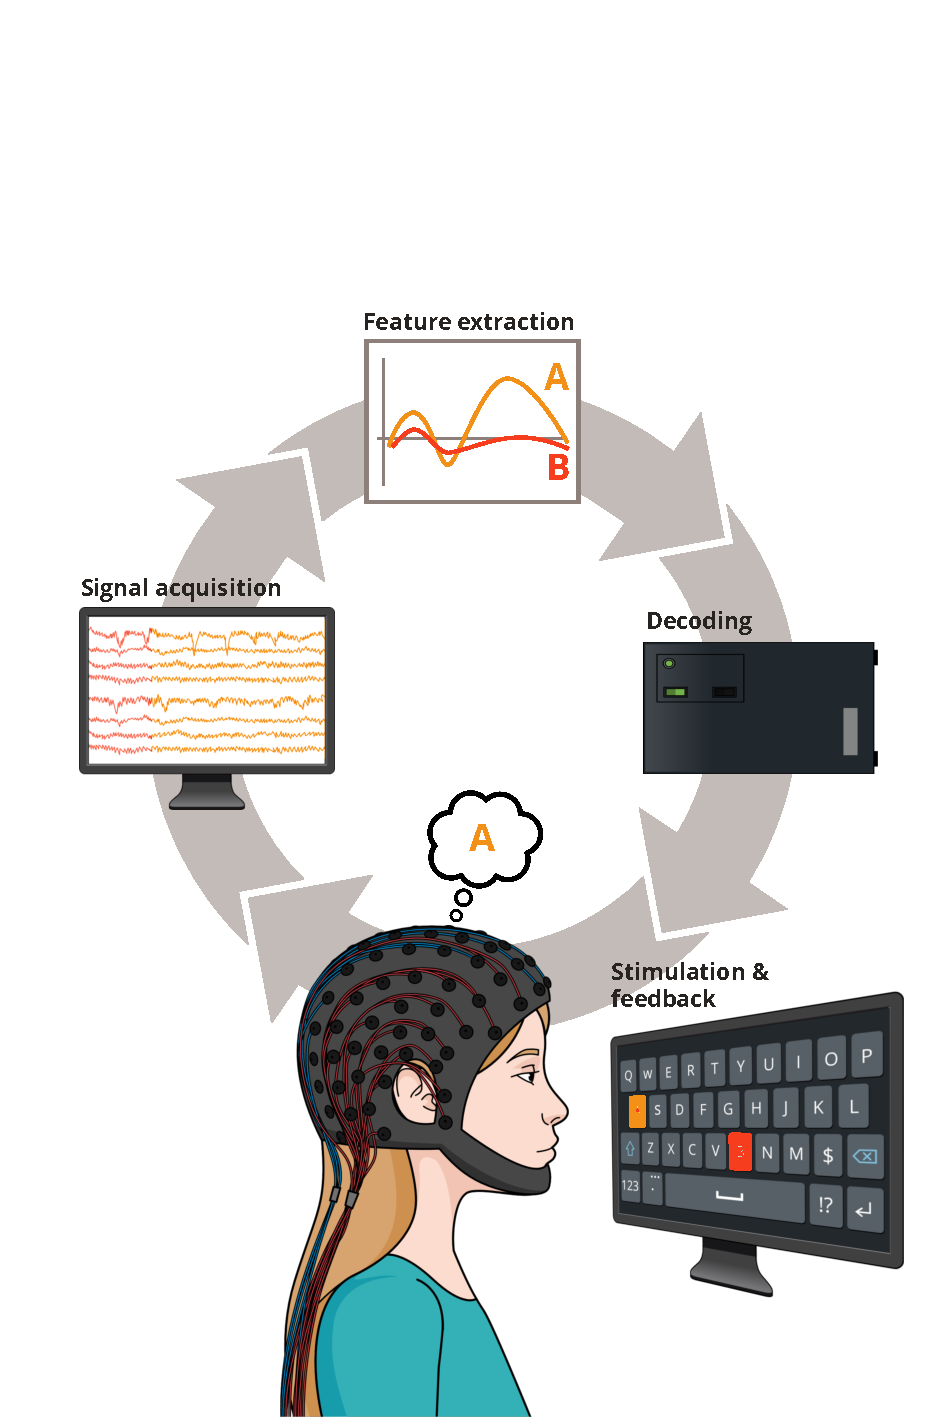
\includegraphics[width=\textwidth]{figures/bci/bci_loop.pdf}
}{%
  The \ac{bci} loop.
  The user interacts with the \ac{bci} via a specific paradigm, in this case involving
  visual stimulation.
  Electrical neural signals are recorded, and neurophysiological features
  related to the paradigm are extracted. Using machine learning, a decision can
  then be made based on these features, which can be presented back to the user.
  In a closed-loop \ac{bci}, this feedback allows the user to adapt to the \ac{bci}.
}{%
  fig:bci/loop
}

Let's break this definition down and focus on its separate parts.
First of all, we need to identify a signal that is a direct representation of
what's going on in the brain.
Section~\ref{sec:bci-recording} gives an overview of the available options.
One might for instance measure the fluctuations in bloodflow to establish the
activity of a specific brain region
However, this signal reacts too slowly to reflect the real-time activity that is
of interest for our purposes, and it carries little information other than the
brain regions where it is originating.
A better candidate is the neuronal electrical activity.
The brain contains 86 billion neurons, which are highly interconnected cells that are
the smallest units of information processing.
The \emph{action potential} and its related \emph{postsynaptic potential}
is an electrical pulse occurring when a neuron receives
input from another neuron and is activated.
The firing of a neuron, or the combined firing of groups of
synchronized neurons, thus generate an electrical field in and near the brain,
which can be measured using electrodes.
Fluctuations in the brain's electrical activity are be faster and more
informative.

The recorded brain waves form only one part of the interaction scheme presented
in Figure~\ref{fig:bci/loop}.
It would make little sense to start digging around at random in all the brain
activity to try to extract the desired output.
It would help greatly if we knew what we are looking for.
For this reason, a \ac{bci} operates using a defined \emph{paradigm}, the manner in
which interaction is performed.
This usually means that the user is instructed to perform a specific task, like
attending a specific flickering stimulus.
We can now exploit background knowledge from prior neuroscientific research
that the brain response evoked by attended stimuli is different of those
unattended,
and determine which one of a set of targets was attended.
In turn, this can be coupled to an action, like typing the inteded letter A or B
in Figure~\ref{fig:bci/loop}.
The \ac{bci} paradigm comprises, if applicable, the manner of stimulation and the
exact task performed by the user, and is often closely linked to the manner of
feedback in the case of a closed-loop system.
As shown in Section~\ref{sec:bci/paradigms}, there is a wide variety of \ac{bci}
paradigms based on different systems in the brain.

The previous points to another component of a successful \ac{bci}: the specific
brain signatures related to our paradigm need to be identified within the recorded
activity.
This is commonly referred to as \emph{feature extraction}.
In other words, the signal needs to be interpreted \emph{in function of} the
task we want our \ac{bci} to perform.
The electrical activity of the brain is relatively weak compared to that of the
environment around us, containing electronic devices and other sources of
interference.
Furthermore, the brain is continuously processing information and carrying out
`background tasks', all of which generate their own brain activity.
On the other hand, the activity of interest often
originates from a specific region or network within the brain.
This activity might not easily be discerned from all other brain and
environmental activity.
Compare this to trying to listen to a single speaker at a noisy party where
everyone is shouting over each other.
Some obvious sources of interference can be easily filtered out by
\emph{preprocessing} (see Section~\ref{sec:bci/preprocessing}), but the problem of retrieving or \emph{decoding} only the
relevant signal is generally hard.
Nevertheless, we can attempt to solve it through supervised machine learning.
Useful information that is encoded in the brain signal by the paradigm,
can be retrieved from it by the decoder.
Section~\ref{sec:bci/decoding} takes a closer look at some common decoding
techniques.

Finally, the loop can be closed by coupling this to a
device or actuator.
There are two aspects to this.
On the one hand, the \ac{bci} gains its function by allowing the user to interact
with their environment.
For a communication system, this means coupling the decoded information to
e.g.\ a virtual keyboard or speech synthesizer.
On the other hand, the actions performed by the \ac{bci} can themselves alter
the user's cognitive state or brain activity, creating an adaptive system.
A direct form of closed-loop \ac{bci} is the use of a neurostimulator.
Examples of this are deep brain stimulation to mitigate the symptoms of
Parkinson's disease, or the cochlear implant as a hearing prosthesis.
More indirectly, modulation can be achieved by sensory stimulation.
This involves specific, paradigm-related sensory input, like tactile
feedback for movement \ac{bci}~\cite{Flesher2021}, or simply presenting selected actions
back to the user.
The user's brain will then adapt through reinforcement learning, causing
changes in behavior or strategy.
Neuroplasticity, the brain's ability to adapt and reinforce specific neural
pathways, can have a positive impact on \ac{bci} performance and gives rise to
rehabilitation applications.
\todo{is every section referred to?}

\todo{wrap-up}
\todo{make shorter}

\section{Recording technologies}
\label{sec:bci-recording}
\todo{why is spatial resolution a good thing}
\todo{explain with each method what it actually is (e.g.\ electrodes placed
at...)}
\todo{make sure every part ends with a short summary motivation for why we chose our
approach}


The brain's activity can be recorded using various neuroimaging
technologies.
These can range from brain scans~\cite{Weiskopf2004} using functional magnetic resonance imaging
(fMRI) to more portable technologies like acoustic signals obtained by functional ultrasound imaging
(fUS)~\cite{Zheng2023} and near-infrared spectroscopy
(fNIRS)~\cite{Borgheai2020}.
The technologies above all measure the hemodynamic signal, which only indirectly
reflects brain activity.
Because of the desirable high temporal resolution~\cite{Easttom2021} and
practicality electrophysiology, we will focus only on methods to record
electromagnetical activity originating from neuronal action potentials.
The magnetical field of the brain can be measured using magnetoencephalography
(MEG)~\cite{Mellinger2007}.
While MEG is non-invasive and results in high-quality signals, the necessary
equipment is rather expensive and impractical.
Recent advances have been made using optically pumped magnetometers
(OPM-MEG)~\cite{Wittevrongel2021}, but this technology still falters outside of
lab conditions.

As a consequence, the \ac{bci} field relies heavily on the
electrical activity of the brain.
As touched upon earlier,the \emph{invasiveness} of the technology forms an
important concept in determining its suitability for a given application and
patient.
As illustrated in Figure~\ref{fig:bci/recording}, invasive electrodes can often measure a very specific brain region and can result in better signal quality, at the cost of the risks
involved with brain surgery.

\fullpagefig{%
  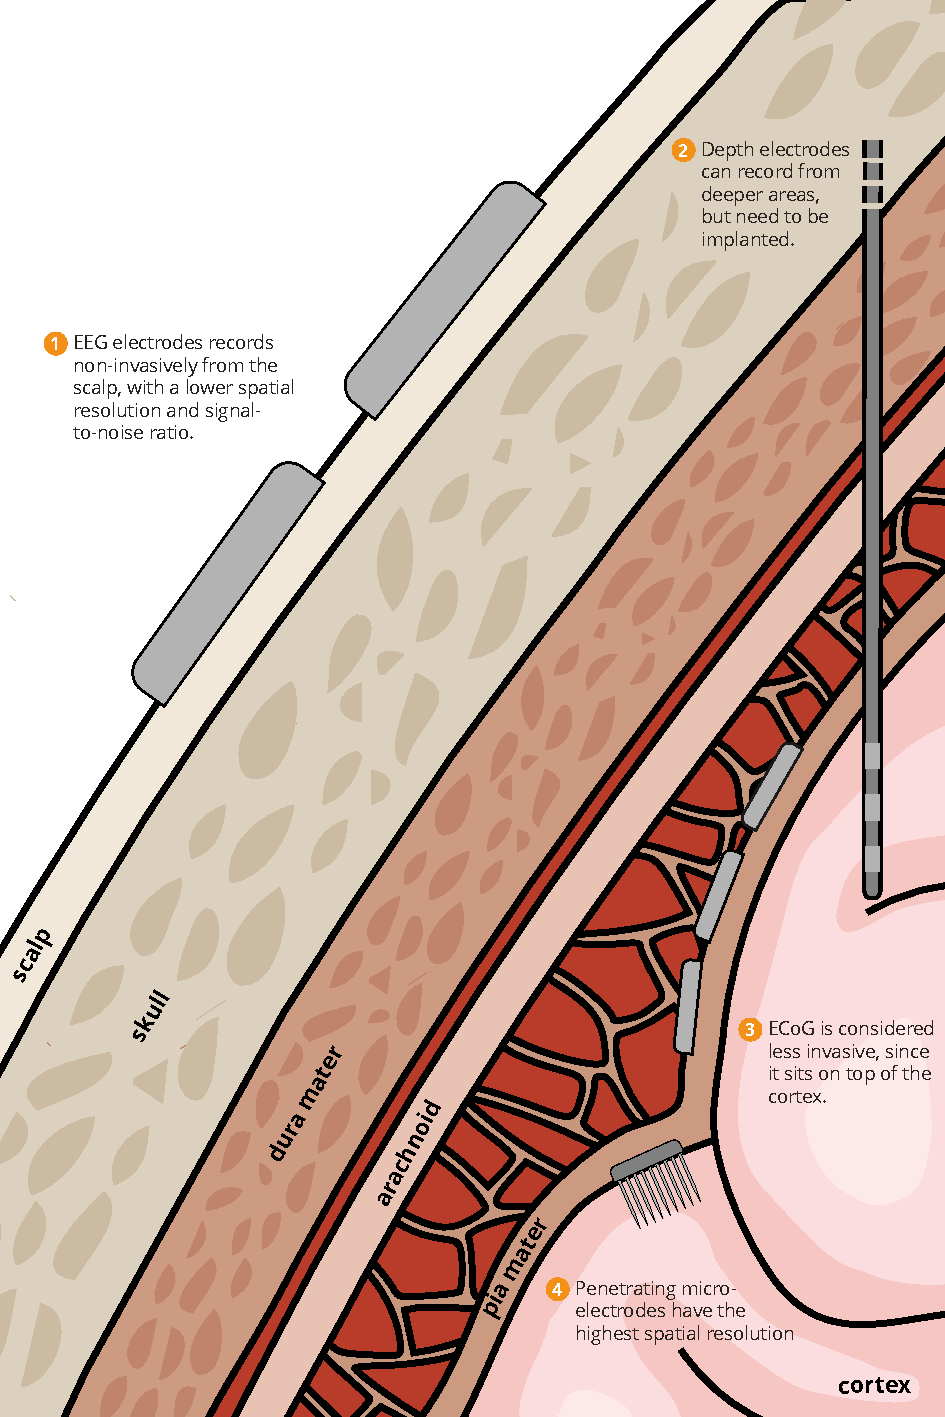
\includegraphics[width=\textwidth]{figures/bci/recording_modalities.pdf}
}{%
	Different electrophysiology recording modalities and \\
	their respective position in a cross-section of the skull. \\
	There is a trade-off between invasiveness and  \\
	spatial resolution.
}{%
  fig:bci/recording
}

Specifically, invasive methods come with an increased \emph{spatial resolution},
meaning they can extract a signal from a specific brain region or even a set of
neurons of interest.
Generally, penetrating microelectrodes are considered to have the highest
spatial resolution.
Microelectrodes can measure the Local Field Potential (LFP), the extracellular
potential of a small group of neurons, or even intracellular single neuron
action potential spikes.
They come in single-electrode form, or, more popularly, in microelectrode
arrays.
Well-known examples are the Utah array~\cite{Maynard1997} and the more recent
NeuraLink implant~\cite{Musk2019} and IMEC's Neuropixels
2.0~\cite{Steinmetz2021}.

Larger implanted electrodes are referred to as intracranial \ac{eeg} (i\ac{eeg}).
Depth electrodes such as those used in stereo-ac{eeg} \ac{bci}~\cite{Wu2024} tasks
and closed-loop adaptive control for Deep Brain Stimulation to mitigate
Parkinson's disease symptoms~\cite{Arlotti2018}.
Since these still penetrate the cortex, electrodes that sit on top of the
cortex are more popular, as they are considered less invasive.
\Ac{ecog} is a powerful method
with many applications in \ac{bci}~\cite{Schalk2011} and epilepsy diagnosis.
Newer developments like micro-ECoG (µECoG)~\cite{Shokoueinejad2019} with a
higher number of smaller electrodes per surface area allow for more precise
measurements.

Some impressive recent breakthroughs in speech and motor \ac{bci} for communication
have been realized using
invasive mictroelectrode arrays~\cite{Willett2021} and $\mu$\Ac{ecog}\cite{Metzger2023}.
Furthermore, recent advances in recording technology focus on improving implant
durability and resolution~\cite{Steinmetz2021}, and on balancing the invasiveness
tradeoff by finding new, minimally invasive ways to record from closer to the cortex.
The Synchron Stentrode~\cite{Mitchell2023}, for instance, can be delivered
through the bloodstream via a catheter, removing the need for open brain
surgery.
Nevertheless, surveys~\cite{Huggins2011, Huggins2015, Branco2021} in different
potential communication \ac{bci} user groups consistently show that non-invasive
technology is preferred over implanted electrodes, unless the added value of invasive BCI is
sufficiently large~\cite{Kageyama2020}.\todo{due to what reasons}
This provides justification for focusing part of the current research effort on
non-invasive BCI.

\Ac{eeg} is the de facto non-invasive electrophysiology standard in clinical
neurology practice as well as in \ac{bci} research.
Developed since 1924~\cite{Berger1929}, it is cheap and relatively practical and
offers great temporal resolution up to thousands of Hz.
\Ac{eeg} measures the electrical potential over time at a given electrode relative to a
reference electrode in volt (V), often on the scale of microvolt ($\mu$V).
As it is easily applicable on the outside of the scalp, many practical
consumer-grade \ac{eeg} headsets exist in the form of (often wireless) electrode
caps or helmets.
Current consumer systems sometimes feature dry electrodes, but clinical and
research systems often use active electrodes with preamplifiers and
electrolyte gel to reduce impedance for improved signal
quality, which slightly decreases practicality, since they require a trained
individual to properly administer.
Nevertheless, it is the most accessible \ac{bci} technology for both patients
and researchers.

The major drawback of \ac{eeg} is its poor spatial resolution.
The electrodes are large and sit on the outside of the scalp, relatively far
away from the cortex.
Furthermore, the layers of skull and cerebrospinal fluid in between can
attenuate the signal and cause volume conduction, which results in electrodes
measuring a mixture of activity from sources elsewhere in the brain.
This also has a negative effect on spectral resolution.
The noise problem mentioned earlier is also prominently present in \ac{eeg}
recordings.
In addition to picking up brain activity other than that of the region of
interest, \ac{eeg} also records other artifacts, from the environment, the power
supply, nearby electrical equipment, or the user's muscle movements.
Combined, this means \ac{eeg} is inherently noisy.
\todo{citations from 'Decoding covert speech from eeg-a cromprehensive review
EEG has lower signal-to-noise ratio (SNR) than the other
modalities. It is almost always corrupted by artifacts such as
muscular artifacts (Eberle et al., 2012; Liu, 2019).
• EEG has limited spectral and spatial resolution (Peled et al.,
2001; Lakshmi et al., 2014).
• Recording EEG for longer duration is challenging since the
conductive gel or the saline solution applied for reducing the
electrode impedance dries up over time, thus increasing the
electrode impedance (Guger et al., 2012; Xu et al., 2018a).
• A trained personnel is required for placing the EEG
electrode cap}

Despite its noisy nature, \ac{eeg} is the recording methodology of choice for
our \ac{bci} because of its wide acceptance by patients.
To counteract the noise present in our recording, we must on the one hand evoke
strong, informative brain signals using a suited \ac{bci} paradigm, and on the
other hand pick a suited decoder which can isolate the signal of interest and
filter out the noise.

\section{\Ac{bci} paradigms}
\label{sec:bci/paradigms}

The \ac{bci} paradigm~\cite{Xu2021,Neeling2019} is the key to translating brain activity into useful
output actions, since it defines which neural responses will be elicited and
captured as features.
A paradigm can be loosely seen as \emph{a way of interacting with the
\ac{bci}}.
According to \textcite{Zander2011}, they can be arranged by their reliance on
external stimulation and the engagement of the user as shown in
Figure~\ref{fig:bci/paradigms}.

\fullpagefig{%
  \sffamily
\begin{tikzpicture}[
    scale=\textwidth/3cm,
  ]
  \useasboundingbox (-1,-1.25) rectangle (1,1);
  \pgfmathsetmacro{\margin}{.1}
  \pgfmathsetmacro{\center}{.5+.5*\margin}
  \pgfmathsetmacro{\textspacing}{.15}
  %\begin{scope}[shift={(1,1.2)}]
    % Draw axes
    \draw[darkgray, very thick, <->] ({-(1+\margin)}, 0) -- ({1+\margin},0);
    \draw[darkgray, very thick, <->] (0,{-(1+\margin)}) -- (0,{1+\margin});

    % Draw rectangles
    \draw[draw=accent1, fill=white, very thick] ({-\margin}, \margin) rectangle (-1,1);
    \draw[draw=accent2, fill=white, very thick] (\margin, \margin) rectangle (1,1);
    \draw[draw=accent3, fill=white, very thick] (-1, {-\margin}) rectangle (1,-1);

    %% Add text
    \node[color=accent1, align=left,font=\bfseries, anchor=north west, inner sep=2pt] at  (-1,1){active};
    \node[color=accent2, align=left,font=\bfseries, anchor=north east, inner sep=2pt] at  (1,1){reactive};
    \node[color=accent3, align=left,font=\bfseries, anchor=south west, inner sep=2pt] at  (-1,-1){passive};

    \node[color=darkgray, align=center,font=\bfseries, anchor=north] at
    (0,{-(1+\margin)}) {passive\\participation};
    \node[color=darkgray, align=center,font=\bfseries, anchor=south] at
    (0,{1+\margin}) {active\\participation};
    \node[color=darkgray, align=center,font=\bfseries, anchor=east] at ({-(1+\margin)}, 0) {stimulus\\independent};
    \node[color=darkgray, align=center,font=\bfseries, anchor=west] at ({1+\margin},0) {stimulus\\dependent};

    %% Text in rectangles
    \node[align=center,font=\small, color=muteblack] at ({-\center}, {\center+1.5*\textspacing}) {motor\\imagery};
    \node[align=center,font=\small, color=muteblack] at ({-\center}, {\center}) {imagined\\speech};
    \node[align=center,font=\small, color=muteblack] at ({-\center}, {\center-1.5*\textspacing}) {neurofeedback};

    \node[align=center,font=\small, color=muteblack] at ({\center+\textspacing}, {\center+\textspacing}) {P300};
    \node[align=center,font=\small, color=muteblack] at ({\center+\textspacing}, {\center-\textspacing}) {SSVEP};
    \node[align=center,font=\small, color=muteblack] at ({\center-\textspacing}, {\center+\textspacing}) {cVEP};
    \node[align=center,font=\small, color=muteblack] at ({\center-\textspacing}, {\center-\textspacing}) {mVEP};

    %% More text
    \node[align=center,font=\small, color=muteblack] at ({\center}, {-\center+\textspacing}) {error\\potentials};
    \node[align=center,font=\small, color=muteblack] at ({-\center}, {-\center+\textspacing}) {attention and \\ workload detection};
    \node[align=center,font=\small, color=muteblack] at ({-\center}, {-\center-\textspacing}) {clinical neuroimaging \\ and monitoring};
    \node[align=center,font=\small, color=muteblack] at ({+\center}, {-\center-\textspacing})  {emotion \\ detection};
  %\end{scope}
\end{tikzpicture}

}{%
  A \ac{bci} paradigm defines which brain activity will be used for control.
  They can be categorized in active, reactive and passive
  paradigms, depending on their reliance on external stimulation and active
  participation required from the user.
  Adapted from~\textcite{Muehl2014}.
}{%
  fig:bci/paradigms
}
\todo{check permissions}
\todo{above Zander and Kothe was mentioned.}

Paradigms that require little active participation of the user like
redirecting attention or initiating imagined actions are classified as \emph{passive
\ac{bci}}.
From the user's point of view, this concept is probably the most attractive,
since their intentions or cognitive state state would be inferred from just
their brain activity.
However, without active user participation, it can be hard to establish reliable
communication or control.
Therefore, passive \ac{bci} are currently more suited to tasks like
emotion or affect monitoring~\cite{Torres2020,Libert2019}, workload
monitoring~\cite{Zanetti2021} or, more dependent on stimulation, error
detection~\cite{SiMohammed2020}.\todo{mention neurofeedback}
Furthermore, active paradigms\todo{"active" is used in a fuzzy way: active BCI is self-paced, reactive is in response to a cued event. Further down that becomes more clear.
The "active participation": is needed in both cases as shown in Fig. 1.3.
I suggest to say active participation} make it easier to quickly collect training data for
supervized machine learning since the conditions can be more easily controlled
by the user or the stimulation.

Paradigms with high active participation can be split up in \emph{active
\ac{bci}} and \emph{reactive \ac{bci}}.
Active \ac{bci} paradigms encode endogenous activity initiated by the user,
such as imagined movement or imagined speech.
These tasks can encode complex information, but current non-invasive
communication methods often limit the considered domain to a few movement
directions to control a cursor, or a few words~\cite{Panachakel2021}.
Invasive recordings are necessary for decoding more complex encoded
like natural speech~\cite{Metzger2023} or meaningful motor trajectories, like handwritten
symbols~\cite{Willett2021} or sign language~\cite{Branco2017}.
Active paradigms are also subject to large inter-subject variability due to the
complexity of the performed tasks.
Imagined speech or movements can be performed in a multitude of ways, which
can each have different neural representations for separate individuals.
This can make it hard to adapt the \ac{bci} to specific individuals, causing
poor performance and giving rise to the concept of \ac{bci}
illiteracy~\cite{Allison2010}\footnote{%
  \cite{Becker2022,Thompson2019}
}.
\todo{footnote on how this just means it needs to be more adapted,
inclusivity, harmful to progress, paraphrase abstracts of articles}
\todo{user training more than with reactive, task instruction}

Reactive \ac{bci} take another approach, by providing a discrete set of
sensory stimulations towards which the user's attention can directed.
Compared to active \ac{bci}, reactive paradigms usually require higher effort
and can induce fatigue due to the constant stimulation.
These paradigms are also somewhat less intuitive compared to e.g.\ speech, and
their expressive power is limited by how many different stimuli can effectively
presented and attended within a reasonable timeframe.
Nevertheless, reactive \ac{bci} work well with \ac{eeg} recordings, and, most
importantly, they work for most people~\cite{Allison2010a,Edlinger2014}.

Reactive \ac{bci} can be realized in multiple ways, depending on the
stimulation used.
Some examples include the following:
In the steady-state somatosensory evoked potentials paradigm~\cite{Petit2021},
the user can attend to one of multiple vibrotactile stimulations in different
limbs, which encodes the information of the attended limb in the brain signal.
In auditory paradigms, information can be modulated by the volume, tone, pitch,
spatial origin of presented sounds, to which the user can
attend~\cite{Kaongoen2017}.
Most common are the visual paradigms.
These can be more performant since they allow the user to use their visual
system, one of the most evolved sensory system in humans.

The major visual paradigms rely on
\ac{ssvep}, \ac{cvep}, oddball and \ac{mvep} brain responses.
In \ac{ssvep}, information is modulated by the frequency of a stimulus attended
among many that each flicker continuously at different
frequencies~\cite{Chen2021}.
In \ac{cvep}, the stimuli flicker instead with distinct on-of patterns, which can
be correlated with the brain activity to retrieve the attended stimulus.
Instead of stimulating all possible selections at once, the oddball paradigm
stimulates them one by one with single flashing.\todo{reference}
Since the times of stimulation of each target is known, and time-points at
which an attention signature is detected to selected targets.
\Ac{mvep} is usually similarly time modulated, but stimuli make sudden
movements in specific directions instead of flashing.
Information is then also carried by movement
direction~\cite{Libert2021a,Libert2022}.


The \ac{bci} paradigms mentioned above can also be combined to gain performance.
Straightforward examples are activating or deactivating \ac{ssvep} stimulation
with a motor command~\cite{Neeling2019}, or combining multiple visual paradigms by stimulating
along multiple dimensions at once.
\textcite{Han2023} recently used this strategy, combining frequency and phase
coding in \ac{ssvep} with the \ac{mvep} and oddball paradigms to develop an
efficient \ac{bci} where one of 200 targets can be accurately selected with
only 800ms of stimulation.

\section{Preprocessing}
\label{sec:bci/preprocessing}
\todo{preprocessing}
EEG preprocessing is a critical step in brain-computer interface (BCI) systems, as it
significantly improves the quality of the recorded data for subsequent analysis and
classification. Common preprocessing techniques in BCI systems include
rereferencing, band-pass and notch filtering, and \ac{ica}.

Rereferencing is an essential first step, where the potential of each EEG channel is
recalculated relative to a common reference point, such as the average of all
electrodes (common average reference) or a selected neutral set of electrodes.
This technique helps reduce noise common across all channels, improving signal clarity
and enhancing the accuracy of subsequent processing steps.

Band-pass filtering is then usually applied to isolate the frequency ranges of interest by
removing frequencies that are too high or too low to contain relevant neural signals.
Band-pass filters eliminate slow drifts and high-frequency noise, such as
muscle artifacts or environmental electrical interference, improving the
\ac{snr}.
Additionally, notch filtering can be  used to remove strong power line
interference\footnote{Typically at 50Hz in Europe}.
This interference can heavily contaminate EEG recordings and even leak through
when outside the passband of a previous filter.
Notch filtering efficiently attenuates this narrowband noise without affecting
the surrounding frequencies.

Finally, to address artifacts like eye blinks and saccades that can significantly
distort the EEG signal, \ac{ica} is
performed~\cite{Delorme2007}.
\Ac{ica} is a blind source separation technique that decomposes the EEG data into
statistically independent components. Components corresponding to eye movements
, blinks and other bodily or environmental artifacts can be identified, either
visually tased on their characteristic topographies and time courses, or
statistically, and then removed.
This leads to cleaner data for subsequent processing, especially in the case of
visual \ac{bci} paradigms.
Since eye movement plays a role in the paradigm, it can strongly be present in
the signal and correlate with the task, forming a confounding factor for
studying control based solely on brain activity.

Together, these preprocessing steps ensure that only the relevant neural signals are
passed on to the feature extraction and classification stages in BCI applications,
improving the accuracy and reliability of the system.

\section{Decoders}%
\label{sec:bci/decoding}

After preprocessing and extracting features, machine learning algorithms can perform \ac{bci}
decoding.
Machine learning decoders use some training data for which the performed tasks
are known, and learn to recognize the activity elicited by the task in recorded data.
The training data can be either obtained from the \ac{bci} user themselves or from
other users.
In the first case, the user would perform a short calibration session before
using the \ac{bci}, where they are instructed to perform a known task.
This calibration session can be eliminated by training the decoder on
preexisting labeled data from other sessions and users, but this is harder due
to the variability between subjects and sessions.

If the goal is to eliminate the per-session calibration, one can also use a
decoder pre-trained on an existing dataset of the same task.
This is complicated by large variability in measured brain response between subjects
and even between different sessions within the same
subject~\cite{Guger2009,Saha2020}.
Therefore, pre-trained decoders must either be trained on a very large, diverse
sample of subjects, or some form of transfer learning must be applied.
Nevertheless, in practice pre-trained models or models using transfer learning often still
require some per session fine-tuning, which still necessitates some
calibration.
Instead, rather opt for keeping the calibration time as short as possible by using
an algorithm that can learn from very few training samples.
This can work well, but requires strong regularization~\cite{VanDenKerchove2022}.

Decoder choice is heavily dependent on constraints set by the paradigm and the
application.
The number of output degrees of features, the serial or parallel nature of
performed tasks, whether the paradigm is active or reactive, etc.\ all need to
be taken into account.
On of these choices is to solve a \emph{regression} or \emph{classification}
problem.
In regression, a continuous output variable is predicted for a new sample,
while classification attempts to sort it into one of a set of discrete classes.
Regression can be useful in \acp{bci} in applications like mapping imagined
movement to an external robot arm.
For communication \acp{bci}, however, conveying information in a symbolic
manner is often of interest.
Many applications resemble virtual keyboards or map a user's actions to
discrete words, predefined actions or letters for full control.
Hence, such problems often present themselves as classification tasks.

\textcite{Lotte2018, Xu2021} present a relatively recent overview of state-of-the art
classification algorithms for decoding.
Classic linear methods, such as \ac{csp} feature extraction for
motor imagery~\cite{Park2017} and \ac{cca} for \ac{ssvep}~\cite{Nakanishi2017},
and \ac{lda} for \ac{erp} classification~\cite{Sosulski2022} still perform
relatively well, given some regularizing constraints or extensions.
Multi-linear techniques exploiting the tensor structure of neural signals are
also promising~\cite{Lotte2018}.
Riemannian Geometry~\cite{Barachant2014} is a popular and robust new strategy.
Furthermore, they lend themselves well to application like adaptive
learning~\cite{Benaroch2021} or transfer learning~\cite{Zanini2017}.
Riemannian Geometry classifiers are often considered the current
state-of-the-art.
Finally, deep learning~\cite{Bhuvaneshwari2021} is also sometimes considered,
albeit only when sufficiently large training datasets are available.
If decoders tailored to a specific user that keep the calibration session as
short as possible are of interest, not enough training data is available to
properly train a deep learning model.

Usually, a decoder makes a prediction for a given \emph{trial} while operating
the \ac{bci}.
A trial is the smallest unit on which a selection decision can be made, for
instance be one imagined movement, or one repetition of flashing all targets
in a visual \ac{erp} \ac{bci}.
Accuracy is a valuable metrics to asses decoder performance in the classification
case.
Accuracy is calculated as the proportion of correct selections to all
selections made.
It should be carefully interpreted in the presence of imbalanced data and always compared to the
random chance accuracy level in the presence of more than two possible
selections per trial.
Alternatively, \ac{rocauc} is also a measure of classifier predictive power, but is more
suited for evaluation of classification of single epochs of data and in the
presence of imbalanced data, e.g.\ when comparing single \acp{erp}.
Higher \ac{rocauc} usually translates to a higher target selection accuracy.

\todomvh{"trial" could  be confused with intensification rounds e.g.}
\todo{remove trial alltogether}
Finally, an important concept in the evaluation of a \ac{bci} decoder, and of \acp{bci}
in general, is \ac{itr}.
\Ac{itr} reflects how fluently a \ac{bci} can be used for communication and can
be calculated as
\begin{equation}
	\text{ITR} = Q\left(\log_2N+P\log_2P+(1-P)\log_2\frac{1-P}{N-1}\right)
\end{equation}
\Ac{itr} is expressed in bits/s and is dependent on $N$, the number of
different options that can be selected per trial\footnote{Given that selections
are independent on each other. This formula requires some adaptations in the
case of sequential or hierarchical selection.}, $P$, the selection accuracy
of the decoder, and $Q$, the number of trials per second.
The parameters $N$, $P$ and $Q$ of this formula give us some insight in the
building blocks a successful, high-\ac{itr} \ac{bci}.
To improve performance, we can aim to
\begin{enumerate*}[label={\arabic*})]
\item increase $N$ by selecting a paradigm and interface that offer a
broad range of informative selections per trial,
\item increase $P$ by engineering more performant machine learning methods for
decoding, and
\item increase $Q$ by selecting a paradigm that allows fast stimulation or
responses.
\end{enumerate*}


\section{A case study: the visual oddball \ac{bci}}

The visual oddball paradigm is a \emph{reactive}, \emph{stimulus-dependent},
\ac{bci} paradigm with all the benefits and drawbacks.
Nevertheless, it can score relatively high on the \ac{itr} parameters established above.
The brain response of interest is the visual \ac{erp}, which can be accurately
measured and decoded from non-invasive \ac{eeg} signals with a relatively low
computational effort and short calibration timeand .
First established by~\cite{Farwell1988} in 1988, it is well supported by literature
and has been proven to work for patients in day-to-day home
use~\cite{Wolpaw2018}.

\subsection{Stimulation paradigm}
One by one, visual elements on a computer screen are \emph{intensified} for a
short period of time by changing in color, brightness or size.
Intensifcations of different targets are usually 100-200ms apart and last for about
100ms~\cite{Sellers2006a}.
On each flash observed by the user, specific brain activity is elicited.
If one of these intensified elements is rare with respect to the others, i.e. it is the
\emph{odd-one out} or \emph{oddball}, this brain activity is altered.
A stimulus can be rare either due to its inherent properties like color or
location.
Crucially, this is also the case if it is `marked' as rare by the user, e.g.
by paying explicit attention to only a given stimulus and not the others or
counting how many times it occurs.
If these visual elements represent letters, and we know the timing of the
intensifications of each letter, we can now establish communication by detecting
for which letter an oddball response was present in the brain signal at its
time of intensification.

\Ac{itr} in the oddball paradigm is optimized by intensifying
multiple targets at once in a row-collumn strategy and using a sequence of
selections, giving rise to the classic matrix speller of~\cite{Farwell1988}.
Other optimizations increase response \ac{snr}, like using flashing face
images as intensifications~\cite{Jin2012} or adding distinct colors and shapes to the
stimuli~\cite{Treder2011}.
The number of targets in a visual oddball \ac{bci} is limited by the crowding
effect, which imposes a limit on how close targets can be to each other while
not distracting the user's attention~\cite{Sellers2006a,Li2010}.
This may be overcome by making hierarchical selections of stimuli representing
groups of selections~\cite{Treder2010}.

Together with \ac{ssvep}, oddball paradigms are most frequently used in visual
\ac{bci}.
There are however indications that users prefer oddball stimulation over
\ac{ssvep} which can cause eye strain and fatigue due to the continuous
oscillatory stimulation of all targets at once~\cite{Xu2021}.
Furthermore, \ac{ssvep} relies more on directing the gaze at the intended
target than oddball, detracting from the concept of control independent from
muscle movement.

\todo{four pane figure:
  photo of someone using a P300 bci
  P300 matrix interface
  simplified figure of ERP components
  full spatiotemporal ERP response
}


\subsection{The \acf{erp}}

The time-domain response elicited immediately after the intensification of a
stimulus is known as the visual \ac{erp}~\cite{Luck2014}.
An \ac{erp} is a waveform consisting of multiple components.
Some of these components are modulated by whether the stimulus was an
oddball or not.
These components appear as positive peaks and negative troughs in the \ac{erp}
waveform.
They follow a naming scheme based on polarity (Negative or Positive) and
latency (e.g., N2 or N200 for a negative component after $\pm200$ ms).
The component most prominently modulated by attention is called the P3
(positive deflection after $\pm300$ ms).\todo{add footnote about how ms naming
is maybe not suited, especially since this work focuses on the fact that there
is a lot of variability in the timings for visual potentials. the short naming
scheme builds on 'the first negative component', 'the first positive
component', and for the visual oddball erp this ordening more or less coincides
with the timings.}
Therefore, oddball paradigms are frequently referred to as P300 paradigms.
However, due to the equally important contributions of other \ac{erp}
components in decoding, as we will show later, this could be considered a
misnomer.
Thus, we will adhere to the oddball paradigm naming.

The visual \ac{erp} components primarily include P1, N1, P2, N2, and P3.
Each component is characterized by specific latency, amplitude, and neural
origins.
These factors influence the perception of visual stimuli and attentional
mechanisms~\cite{Luck2013}.

\emph{The P1 component} occurs approximately 100 ms after stimulus presentation.
This component reflects initial visual processing and is primarily linked to
activity in the primary visual cortex.
P1 is particularly sensitive to gaze fixation, where the gaze is directed
toward a stimulus.
When a stimulus is fixated on, the amplitude of P1 increases, reflecting the
enhanced processing of that visual input.
In contrast, P1 shows less modulation when stimuli are attended to via
attention without direct gaze.

\emph{The N1 component} peaks around 150 to 200 ms post-stimulus.
It represents an extension of sensory processing related to both gaze fixation
and attention.
For attended stimuli, the amplitude is greater, indicating prioritization for
further cognitive processing.
This highlights a more selective form of attention allocation, demonstrating
the impact of both types of attention on visual processing.

\emph{The P2 component} occurs between 200 to 300 ms.
It reflects higher-order processing, particularly in contexts demanding
stimulus evaluation and feature detection.
P2 is sensitive to attention.
When participants actively engage with specific features or categories of
stimuli, P2 shows increased amplitude.
Conversely, P2 may be less responsive when gaze is not directed toward the
stimulus but attention is still maintained.

\emph{The N2 component} peaking around 200 to 350 ms is associated with cognitive
control processes such as conflict monitoring and inhibition.
It is particularly pronounced in tasks requiring differentiation between
competing stimuli.
N2 reflects the allocation of attentional resources required to resolve
conflicts, irrespective of whether the gaze is directly on the competing
stimuli or not.
Higher amplitudes in N2 are seen when cognitive demands increase, indicating
the influence of attention strategies.

\emph{The P3 component} is elicited in oddball paradigms and peaks around 300 ms
post-stimulus.
It reflects attentional engagement and the processing of rare or unexpected
events.
The P3 is typically subdivided into two subcomponents: P3a and P3b.
The P3a is associated with the allocation of attention to novel or unexpected
stimuli, indicating the initial detection of a change in the environment.
It is particularly responsive to stimuli that capture attention, whether
through gaze fixation or attention.
P3a typically exhibits a frontal distribution and peaks earlier than P3b.

Conversely, the P3b relates to the evaluation of the stimulus.
It involves the updating of cognitive resources in response to task relevance.
This subcomponent is typically observed over parietal regions.
P3b is elicited when participants must process the stimulus meaningfully,
often requiring a decision or response.
Both P3a and P3b amplitudes are sensitive to the probability of occurrence
and the participant's attentional focus, showing how attentional strategies
affect cognitive processing.

\emph{The late positive potential (LPP)} is a later component occurring beyond 400 ms.
Sustained attention and emotional processing of stimuli are reflected in the
LPP.
Typically enhanced for emotionally salient or motivationally relevant
information, the LPP serves as an indicator of cognitive appraisal beyond mere
recognition tasks.
This component can be influenced by attention when the participant evaluates
the emotional significance of stimuli, even if gaze is not directed at them.

In summary, ERP components such as P1, N1, P2, N2, P3, and LPP collectively
elucidate the neural underpinnings of visual processing and attentional
mechanisms.
These components not only inform the design of an effective oddball BCI system
but also enhance our understanding of the cognitive processes involved in visual
attention.
This includes both gaze fixation and attention.
Understanding these components is essential for optimizing BCI protocols and
improving user interaction, particularly in contexts involving visual oddball
tasks.

\subsection{Preprocessing}
In addition to (ref) epoching
baseline correction, but not in decoding (cite)


\subsection{Decoding ERPs}

Usually, snr low and multiple trials necessary

tLDA, beamforming
Linear decoding techniques
